\documentclass[border=3pt]{standalone}
% Preâmbulo compartilhado pelos diagramas TikZ da aula 4 de Navegação (Representação de Mapas)
\usepackage[T1]{fontenc}
\usepackage[utf8]{inputenc}
\usepackage{lmodern}
\usepackage{amsmath}
\usepackage{xcolor}
\usepackage{tikz}
\usetikzlibrary{arrows.meta,angles,quotes,decorations.pathmorphing,decorations.pathreplacing,calc,
                positioning,shapes.geometric,shapes.misc,backgrounds,fit,
                math}

% Paleta (mesma dos SVGs originais)
\definecolor{dblue}{HTML}{2A5B8C}
\definecolor{dorange}{HTML}{B3541E}
\definecolor{dgreen}{HTML}{4A7C59}
\definecolor{dred}{HTML}{9C4B4B}
\definecolor{dcream}{HTML}{F4F1EA}
\definecolor{dshade}{HTML}{DDD7C9}

% Função gaussiana (não normalizada por padrão de escala visual)
\pgfmathdeclarefunction{gauss}{3}{%
  \pgfmathparse{1/(#3*sqrt(2*pi))*exp(-((#1-#2)^2)/(2*#3^2))}%
}

% Estilos comuns (prefixo d... para não colidir com chaves internas do pgf)
\tikzset{
  >={Stealth[length=2mm]},
  dguide/.style={gray!55, dashed, line width=0.4pt},
  daxis/.style={gray!60, line width=0.7pt, ->},
  dbody/.style={fill=black!3, draw=black!80, line width=1pt},
  dacc/.style={draw=dblue, line width=1pt},
  dlbl/.style={black!55, font=\small},
  dsub/.style={black!45, font=\footnotesize},
  dstate/.style={circle, draw=black!80, fill=dcream, line width=1pt,
                 minimum size=17mm, font=\large, inner sep=1pt},
  dobs/.style={circle, draw=black!80, fill=dshade, line width=1pt,
               minimum size=14mm, font=\large, inner sep=1pt},
  dbox/.style={rounded corners=2pt, draw=black!80, fill=dcream, line width=1pt,
               align=center, inner sep=6pt},
  dop/.style={circle, draw=black!80, fill=white, line width=1pt,
              minimum size=6mm, inner sep=0pt, font=\small},
  dtrans/.style={->, dblue, line width=1pt},
  dmeas/.style={->, dorange, line width=1pt},
  dcurve/.style={line width=1pt, dblue},
  dcurveb/.style={line width=1.4pt, dorange},
}

\begin{document}
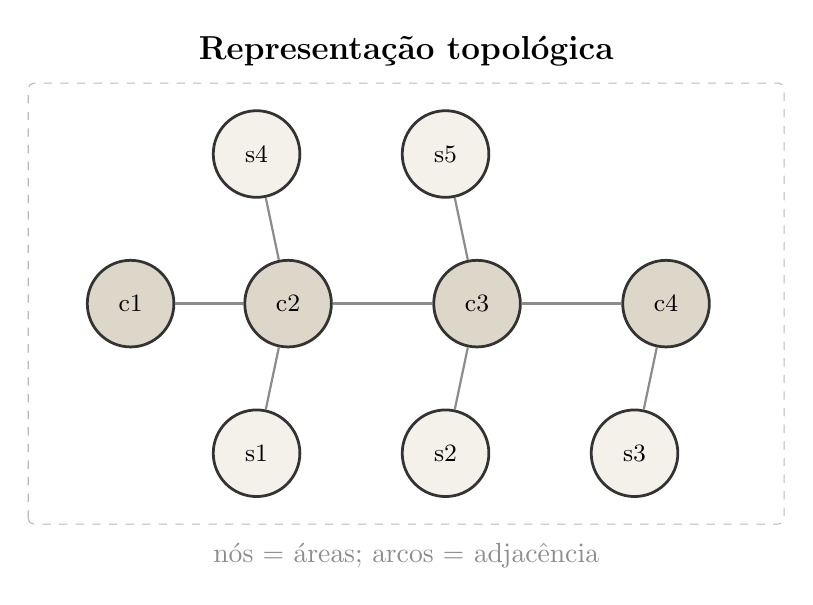
\begin{tikzpicture}[x=1cm,y=1cm]

    \draw[dguide, rounded corners=2pt] (-0.3,-0.3) rectangle (9.3,5.3);
    \node[font=\bfseries\large] at (4.5,5.7) {Representação topológica};

    \node[dobs, minimum size=11mm, font=\small] (c1) at (1,2.5) {c1};
    \node[dobs, minimum size=11mm, font=\small] (c2) at (3,2.5) {c2};
    \node[dobs, minimum size=11mm, font=\small] (c3) at (5.4,2.5) {c3};
    \node[dobs, minimum size=11mm, font=\small] (c4) at (7.8,2.5) {c4};
    \draw[dsub, line width=1pt] (c1)--(c2)--(c3)--(c4);

    \node[dstate, minimum size=11mm, font=\small] (s1) at (2.6,0.6) {s1};
    \node[dstate, minimum size=11mm, font=\small] (s2) at (5.0,0.6) {s2};
    \node[dstate, minimum size=11mm, font=\small] (s3) at (7.4,0.6) {s3};
    \node[dstate, minimum size=11mm, font=\small] (s4) at (2.6,4.4) {s4};
    \node[dstate, minimum size=11mm, font=\small] (s5) at (5.0,4.4) {s5};

    \draw[dsub, line width=0.8pt] (c2)--(s1);
    \draw[dsub, line width=0.8pt] (c3)--(s2);
    \draw[dsub, line width=0.8pt] (c4)--(s3);
    \draw[dsub, line width=0.8pt] (c2)--(s4);
    \draw[dsub, line width=0.8pt] (c3)--(s5);

    \node[dsub, font=\normalsize] at (4.5,-0.7) {nós = áreas; arcos = adjacência};
  \end{tikzpicture}
\end{document}
